\section{ヘッドセットの使い方}
演習の前に、ヘッドセットの設定をしましょう。ヘッドセットとは、コンピュータなどから音声を出力するためのヘッドフォンと、コンピュータなどに音声を入力するためのマイクが一体型になったものです。\\
まずはラズベリーパイの電源を入れる前に、ヘッドセットとラズベリーパイをつないでおきます。

\begin{figure}[H]
\begin{center}
    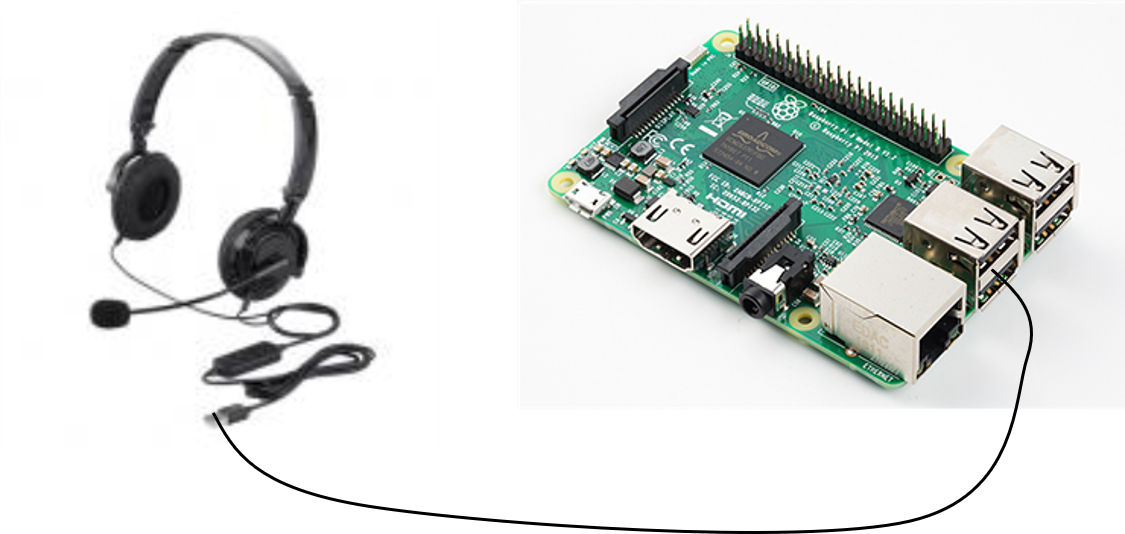
\includegraphics[width=\linewidth]{images/chap06/text06-img003.png}
    \caption{つなげかた}
    \label{つなげかた}
\end{center}
\end{figure}

ヘッドセットの出力音量はコントローラーかディスプレイで調整できます。

\begin{figure}[H]
\begin{center}
    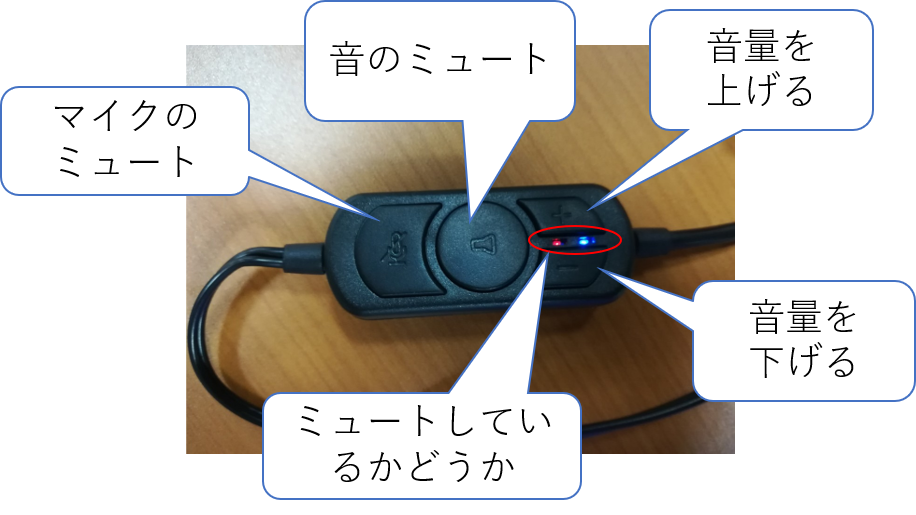
\includegraphics[width=\linewidth]{images/chap06/text06-img004.png}
    \caption{ヘッドセットのコントローラーの使い方}
    \label{ヘッドセットのコントローラーの使い方}
\end{center}
\end{figure}

一番左のボタンでマイクのミュートを切りかえることができます。ミュートとは音を消すことです。マイクがミュートしているときは赤色のLEDが光っています。マイクを使うときはミュートを解除して、赤色のLEDが光っていないようにしましょう。真ん中のボタンは音のミュートです。音が聞こえないときはここを押してみましょう。右側のボタンは”+”で音量を上げる、”-”で音量を下げることができます。

マイクの音量はディスプレイからも設定できます。

\begin{figure}[H]
\begin{center}
    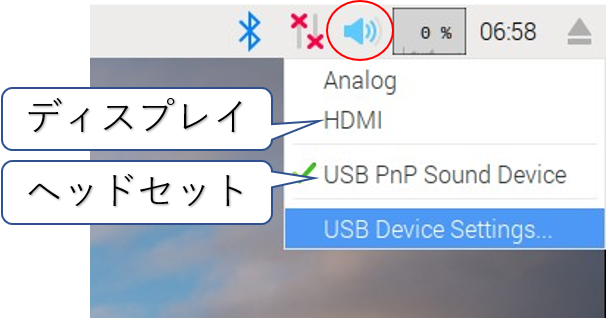
\includegraphics[width=\linewidth]{images/chap06/text06-img005.png}
    \caption{使う音声デバイスの選択と設定}
    \label{使う音声デバイスの選択と設定}
\end{center}
\end{figure}

ディスプレイの右上にある音マークを右クリックしてみましょう。使うことのできるデバイスが表示されます。HDMIとはディスプレイのことです。これを左クリックするとディスプレイから音を出すことができます。教室ではヘッドセットを使いますが、おうちではお父さんやお母さんにいいよと言われたら、ディスプレイやテレビから出力することもできます。USB PnP Sound Deviceはヘッドセットのことです。ヘッドセットを使うときはこちらを左クリックします。\\

音量を変えるときは一番下のUSB Device Settings...を左クリックします。

\begin{figure}[H]
\begin{minipage}[t]{0.3\linewidth}
\begin{center}
    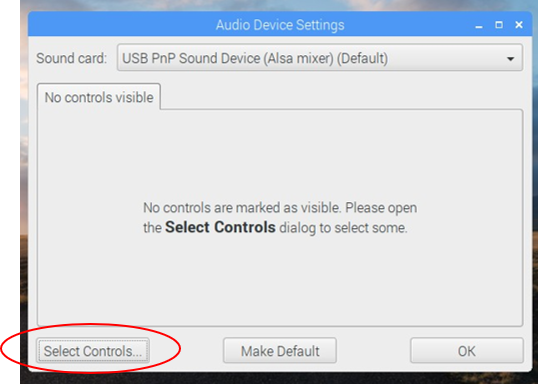
\includegraphics[width=\linewidth]{images/chap06/text06-img006.png}
    \caption{画面の右上の音マークから USB Device Settings... をクリックしたところ。マイクの入力音量を調節するには、Select Controls をクリックする。}
    \label{音量変更1}
\end{center}
\end{minipage}
\begin{minipage}[t]{0.3\linewidth}
\begin{center}
    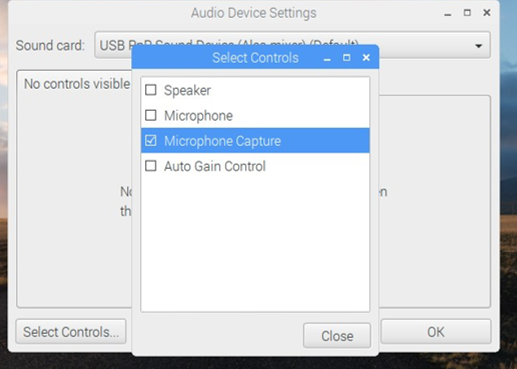
\includegraphics[width=\linewidth]{images/chap06/text06-img007.png}
    \caption{配布したヘッドセットのマイク設定をするために、「Microphone Capture」 をクリック。}
    \label{音量変更2}
\end{center}
\end{minipage}
\begin{minipage}[t]{0.3\linewidth}
\begin{center}
    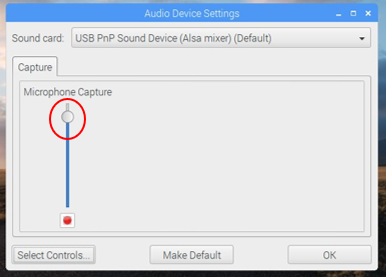
\includegraphics[width=\linewidth]{images/chap06/text06-img008.png}
    \caption{バーを上げ下げしてマイクの音量を調節する。}
    \label{音量変更3}
\end{center}
\end{minipage}
\end{figure}

左下のSelect Controlsをクリックすると、真ん中の画面が出てきます。Microphone Captureをクリックしチェックを付けて画面を閉じます。すると右の画面のように音量調節バーが出ます。丸いつまみを上下に動かすことで音量を調節することができます。

教室ではヘッドセットで音を聞き、ヘッドセットのマイクで音声を入力するので、図\ref{使う音声デバイスの選択と設定}のように USB PnP Sound Device を選択し、図\ref{音量変更3}のようにマイクの入力音量を大きめにしておきましょう。

この際,「Make Default」ボタンを押してしまわないように注意してください.このボタンを押すと異なる設定がされてしまい,後で使う音声認識のプログラムが動作しなくなる場合があります.もし誤って押してしまった場合は,一度  \textasciitilde /.asoundrc を rm コマンドで削除してから,音声デバイスを再度設定してください.すでに使いたい音声デバイスが設定されている場合は,一度他の音声デバイスを選択してからもう一度使いたい音声デバイスを設定してください.たとえば,USB PnP Sound Device を使いたい場合は,一度 Analog を選択してからもう一度 USB PnP Sound Device を設定してください.
